% Section 5: The zero-shot useful-context predictor
% Required packages: \usepackage{amsmath,booktabs,graphicx}
% Upload this file together with the three PDF figures under figures/.

\section{The zero-shot useful-context predictor}
\label{sec:zero-shot-predictor}

Sections~\ref{sec:real-context}--\ref{sec:context-mechanisms} showed that the
best context is neither fixed nor directly observable: it varies across
forecasting problems, responds to genuine distant dependencies, and can trade
accuracy against substantial computation.  This section turns that diagnostic
opportunity into a selection problem.  Instead of estimating a latent memory
length, we learn the \emph{forecast-error response over a discrete context
grid} and choose an operating point from the predicted curve.

The key question is whether that response can be learned without real-domain
error curves.  Our selector is trained only on synthetic series labeled by a
frozen TSFM; no GiftEval series or forecast outcomes enter training or
checkpoint selection.  We first establish the accuracy--compute trade-off on
Chronos2-Small, then test whether the same synthetic-supervision recipe remains
calibrated across 11 forecasters.

\subsection{Synthetic supervision from a frozen forecaster}
\label{sec:zero-shot-labels}

We generate a shared pool of $50{,}000$ synthetic series with one to four
regimes, and each frozen TSFM labels that pool independently.  The generator
varies level, scale, trend, autoregressive dynamics, seasonal period and
waveform, abrupt or gradual transitions, and impulse outliers.  Ten percent of
the pool contains shorter genuine histories, left-padded only at the predictor
input.  The common pool is $15{,}360$ steps wide; predictors for models capped
at $8{,}192$ steps consume its most recent $8{,}192$ values.

The frozen TSFM labels each series at every supported context action
$L_k\in\mathcal{G}_m$ and forecast horizon

\begin{equation}
    h\in\mathcal{H}
      = \{16,32,64,128,512,1024\}.
    \label{eq:predictor-horizon-grid}
\end{equation}

One longest-horizon forecast supplies prefix errors for the shorter horizons.
For Chronos2-Small, $\mathcal{G}_m$ contains 18 suffix lengths from 32 to
8,192.  Other models use the same base grid truncated at their supported
context, with an off-grid native cap added where necessary.  The label is the
complete MAE surface

\begin{equation}
    E^{(m)}_{i,k,h}
      = \frac{1}{h}\sum_{t=1}^{h}
        \left|y_{i,t}
        -f_m\!\left(x_{i,-L_k:}\right)_t\right|,
    \label{eq:synthetic-error-surface}
\end{equation}

not a generator parameter.  Thus the supervisor includes the forecaster's
architecture, preprocessing, and failure modes.  A separate labeled surface
and a separate selector are built for each TSFM; the main experiment does not
assume that the useful-context policy transfers across forecasters.

\begin{figure*}[t]
    \centering
    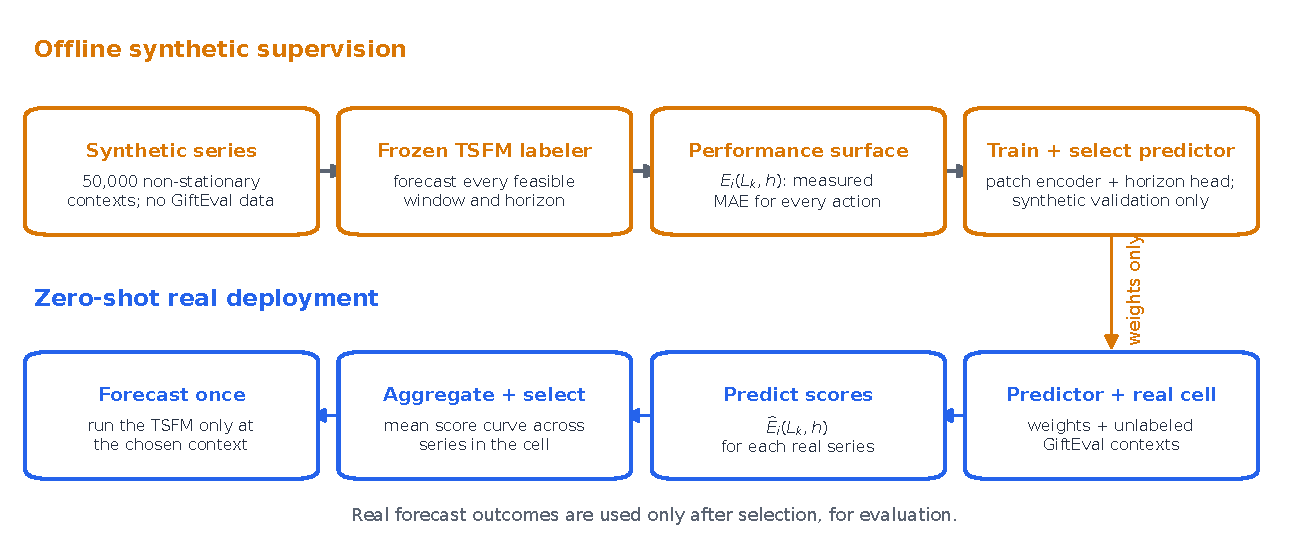
\includegraphics[width=\textwidth]{figures/fig1_zero_shot_pipeline.pdf}
    \caption{Training and deployment of the zero-shot selector.  Offline, a
    frozen TSFM measures the error surface of 50,000 synthetic series over
    context and horizon.  At deployment, the learned predictor scores every
    feasible window from unlabeled real contexts; scores are averaged within a
    dataset--term cell and one context action is selected.  GiftEval forecast
    outcomes are revealed only afterward for evaluation.}
    \label{fig:zero-shot-pipeline}
\end{figure*}

\subsection{Horizon-conditioned curve prediction}
\label{sec:zero-shot-model}

The input series is divided into non-overlapping patches and projected into a
latent sequence.  A learned summary token, augmented by an embedding of the
requested horizon, is prepended before the sequence encoder.  Its final state
is mapped to one score per candidate context.  We study two encoders under the
same input and output interface: a low-capacity Patch-Transformer and a
bidirectional Mamba stack.  The constrained search uses patch lengths 64 or
128, width 128, and two or four layers.  Mamba is linear in the number of patch
tokens, whereas dense self-attention is quadratic.

For curve regression, each synthetic error curve is standardized over its
valid windows,

\begin{equation}
    z_{i,k,h}
      = \frac{E_{i,k,h}-\mu_{i,h}}
             {\sigma_{i,h}+10^{-8}},
    \quad
    \mu_{i,h}=\frac{1}{|\mathcal{V}_{i,h}|}
       \sum_{k\in\mathcal{V}_{i,h}}E_{i,k,h},
    \label{eq:curve-standardization}
\end{equation}

where $\mathcal{V}_{i,h}$ contains the windows that the TSFM can serve.
Standardization removes arbitrary error level and scale while preserving the
argmin.  During training, a random subset of input patches is masked and a
second head reconstructs their raw values.  The loss is

\begin{equation}
    \mathcal{L}
      = \lambda_{\mathrm{curve}}
          \frac{\sum_{i,k,h}M_{i,k,h}
          (\widehat z_{i,k,h}-z_{i,k,h})^2}
               {\sum_{i,k,h}M_{i,k,h}}
        + \lambda_{\mathrm{rec}}
          \operatorname{MSE}_{\mathrm{masked}}(\widehat x,x),
    \qquad
    (\lambda_{\mathrm{curve}},\lambda_{\mathrm{rec}})=(1,0.5),
    \label{eq:predictor-loss}
\end{equation}

with $M$ masking unsupported labels.  The auxiliary reconstruction objective
regularizes the representation; it is not evaluated at inference.

We also test decision-focused targets on Chronos2-Small.  The strongest is a
soft top-$k$ classifier in which the best, second-best, and third-best windows
receive independent binary targets $1$, $1/2$, and $1/4$.  Additional ablations
predict calibrated risk relative to full context, adjacent pairwise
preferences, or the set of actions within $3\%$ of the row oracle.  All
variants retain the same synthetic-only split: 45,000 training and 5,000
validation series.  Thirty random-search trials are ranked by mean synthetic
validation regret,

\begin{equation}
    R_{\mathrm{val}}
      = \mathbb{E}_{i,h}\left[
          \frac{E_{i,\widehat k_i,h}
                -\min_{k\in\mathcal{V}_{i,h}}E_{i,k,h}}
               {\min_{k\in\mathcal{V}_{i,h}}E_{i,k,h}}
        \right].
    \label{eq:synthetic-validation-regret}
\end{equation}

For the selected Chronos2-Small curve model, Mamba uses 64-step patches, width
128, and four bidirectional layers; its synthetic validation regret is 0.1956.

\subsection{Zero-shot decision protocol}
\label{sec:zero-shot-decision}

At real-data inference, the predictor emits a score vector
$\widehat{\boldsymbol{s}}_{i,h}$ for each forecast instance.  We use the same
cell-shared decision granularity as the principal oracle in
Section~\ref{sec:real-context}: for dataset--term cell $c$, the curve-regression
policy selects

\begin{equation}
    \widehat L_c
       = L_{\widehat k_c},
    \qquad
    \widehat k_c
       \in \arg\min_{k\in\mathcal{V}_c}
          \frac{1}{n_c}\sum_{i\in c}\widehat s_{i,k,h_c}.
    \label{eq:zero-shot-cell-policy}
\end{equation}

The classification variant replaces the argmin by the maximum mean predicted
probability.
This aggregation uses cell membership and input contexts, but neither targets
nor realized forecast errors.  It is therefore a batch-level zero-shot policy,
not a fully online per-series rule.  After selecting $\widehat L_c$, the TSFM is
run at that context and scored on the same 97 GiftEval cells and 371,330
instances used in Section~\ref{sec:real-context}.

Accuracy is the normalized MASE in Equation~\ref{eq:normalized-mase}.  The main
compute number is the cell-balanced sum of theoretical TSFM FLOPs, matching the
oracle analysis; measured time sums cached TSFM forward-pass timings.  Unless
stated otherwise, neither number includes selector inference, which we audit
separately below.

\subsection{Accuracy--compute operating points}
\label{sec:zero-shot-chronos}

Chronos2-Small provides the clearest test of whether synthetic supervision can
recover a useful real-data operating point.  Table~\ref{tab:zero-shot-objectives}
compares five objectives selected without GiftEval feedback.  Every learned
policy improves on native context, but they occupy different regions of the
accuracy--compute plane.

The curve predictor is the most compute-efficient policy: it lowers normalized
MASE from 0.726708 to 0.724344 while saving $56.49\%$ of cell-balanced
theoretical TSFM FLOPs and $52.62\%$ of measured forward time.  The soft
top-$k$ classifier reaches the best accuracy, 0.722412 ($0.591\%$ better than
native), with a more conservative $27.89\%$ FLOPs reduction.  Thus the learned
target controls the operating point: curve regression favors aggressive
shortening, whereas rank-weighted classification better protects accuracy.

\begin{table*}[t]
    \centering
    \footnotesize
    \setlength{\tabcolsep}{5pt}
    \caption{Accuracy--compute operating points on Chronos2-Small.  Positive
    $\Delta$ denotes improvement over native context.  FLOPs and time refer to
    the TSFM forecast stage and exclude selector inference.  The hindsight cell
    oracle is included only to show remaining headroom.}
    \label{tab:zero-shot-objectives}
    \begin{tabular}{lrrrrr}
        \toprule
        Policy & nMASE & $\Delta$ & FLOPs saved & Time saved & Wins / 95 \\
        \midrule
        Native/full                    & 0.726708 & --       &  0.00\% &  0.00\% & -- \\
        Mamba curve                    & 0.724344 & $+0.325\%$ & 56.49\% & 52.62\% & 54 \\
        Soft top-$k$ classification    & \textbf{0.722412} & $\mathbf{+0.591\%}$ & 27.89\% & 39.61\% & 46 \\
        Risk-aware                     & 0.726155 & $+0.076\%$ & 57.80\% & 51.27\% & 56 \\
        Adjacent pairwise              & 0.725725 & $+0.135\%$ & 54.24\% & 39.62\% & 58 \\
        $3\%$ acceptable set           & 0.723630 & $+0.423\%$ & 26.39\% & 32.24\% & 46 \\
        \midrule
        Cell-shared accuracy oracle    & 0.704681 & $+3.031\%$ & 53.88\% & -- & 77 \\
        \bottomrule
    \end{tabular}
\end{table*}

Cell wins and aggregate accuracy capture different aspects of the policy.
Pairwise learning improves 58 of the 95 selection-eligible cells, the highest
count in the table, but gains only $0.135\%$ in normalized MASE.  The soft
top-$k$ classifier wins fewer cells yet achieves the best aggregate score,
indicating that controlling the magnitude of harmful selections matters more
than maximizing the raw win count.

Figure~\ref{fig:zero-shot-objectives} locates the learned policies relative to
the hindsight frontier.  The selectors move beyond the native baseline, but a
visible calibration gap remains: at comparable compute, the curve predictor is
$2.78\%$ worse than the oracle, and the classification point is $2.52\%$ above
the minimum-MASE oracle.  The window grid already contains substantially better
actions; the remaining challenge is to rank them reliably from synthetic
supervision.

\begin{figure}[t]
    \centering
    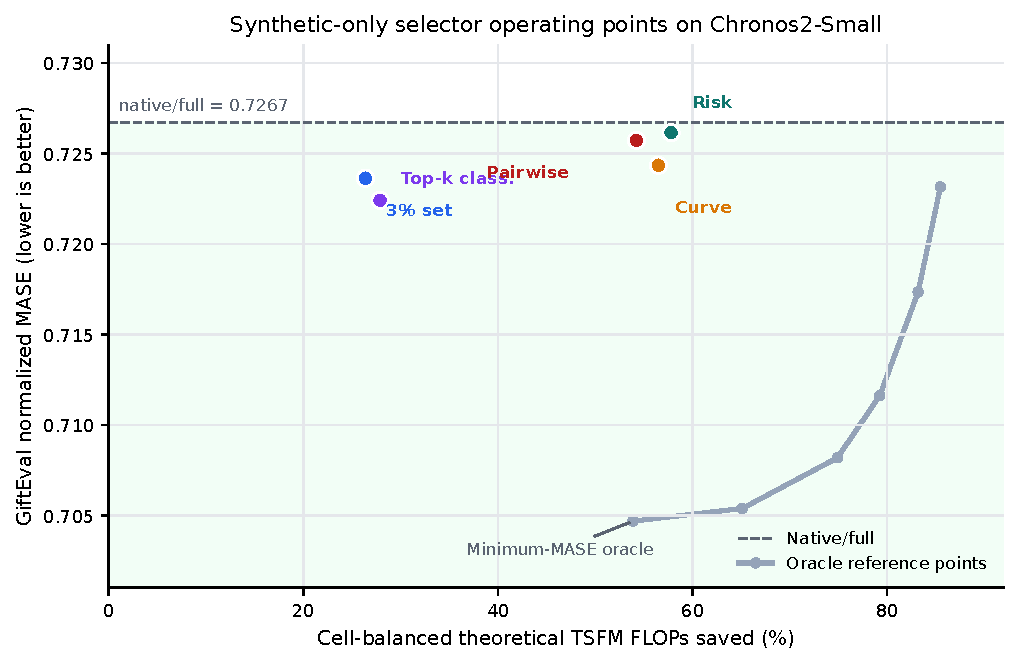
\includegraphics[width=\columnwidth]
        {figures/fig2_chronos_objective_operating_points.pdf}
    \caption{Accuracy--compute locations of the five synthetic-only
    Chronos2-Small selectors.  The gray line joins selected supported oracle
    reference points and is not an attainable zero-shot curve.  Green shading
    marks accuracy better than native/full.  Curve regression and soft top-$k$
    classification occupy complementary compute and accuracy regimes.}
    \label{fig:zero-shot-objectives}
\end{figure}

\subsection{Transfer across forecasters}
\label{sec:zero-shot-multimodel}

We next repeat the complete labeling and curve-training procedure independently
for 11 TSFMs while holding the GiftEval cohort fixed.  The selectors consistently
learn to shorten context, but accuracy transfer is model dependent
(Table~\ref{tab:zero-shot-multimodel}).  Mamba improves native accuracy for
Chronos2-Small and Moirai2-Small.  Moirai gives the strongest transfer result:
normalized MASE falls from 0.737778 to 0.731958 ($0.789\%$) while theoretical
TSFM FLOPs fall by $65.17\%$.  For the other nine forecasters, the learned
policies still reduce context compute but incur accuracy costs between
$0.256\%$ and $1.906\%$.

\begin{table*}[t]
    \centering
    \footnotesize
    \setlength{\tabcolsep}{5pt}
    \caption{Transfer of the bidirectional-Mamba curve predictor across 11
    TSFMs.  Each row uses model-specific synthetic labels and checkpoint
    selection.  Positive $\Delta$ denotes improvement over native context;
    FLOPs savings exclude predictor inference.}
    \label{tab:zero-shot-multimodel}
    \begin{tabular}{lrrrr}
        \toprule
        Model & Native nMASE & Predicted nMASE & $\Delta$ & FLOPs saved \\
        \midrule
        Chronos2-Base       & 0.704738 & 0.706544 & $-0.256\%$ & 32.66\% \\
        Chronos2-Small      & 0.726708 & 0.724344 & $+0.325\%$ & 56.49\% \\
        Chronos2-Synth      & 0.735228 & 0.738399 & $-0.431\%$ & 34.59\% \\
        ChronosBolt-Base    & 0.809586 & 0.820556 & $-1.355\%$ & 27.48\% \\
        FlowState-R1        & 0.709001 & 0.713912 & $-0.693\%$ & 27.28\% \\
        Moirai2-Small       & 0.737778 & \textbf{0.731958} & $\mathbf{+0.789\%}$ & 65.17\% \\
        PatchTST-FM-R1      & 0.704527 & 0.717957 & $-1.906\%$ & 22.98\% \\
        Sundial-Base-128M   & 0.750750 & 0.756259 & $-0.734\%$ & 17.63\% \\
        TiRex2              & 0.696689 & 0.709750 & $-1.875\%$ & 31.41\% \\
        TimesFM2.5-200M     & 0.705040 & 0.713009 & $-1.130\%$ & 46.86\% \\
        Toto-2.0-313m       & 0.703999 & 0.707562 & $-0.506\%$ & 15.99\% \\
        \bottomrule
    \end{tabular}
\end{table*}

The same pattern holds with the low-cost Patch-Transformer
(Figure~\ref{fig:zero-shot-multimodel}): it also improves two models, Moirai and
Sundial, while its largest accuracy cost is $3.01\%$ on PatchTST-FM.  Because
the successful forecasters change with the predictor backbone, encoder choice
alone does not explain transfer.  Synthetic labels contain useful ranking
signal, but the mapping from synthetic response curves to real operating points
must be calibrated for the forecaster as well as the data domain.

\begin{figure*}[t]
    \centering
    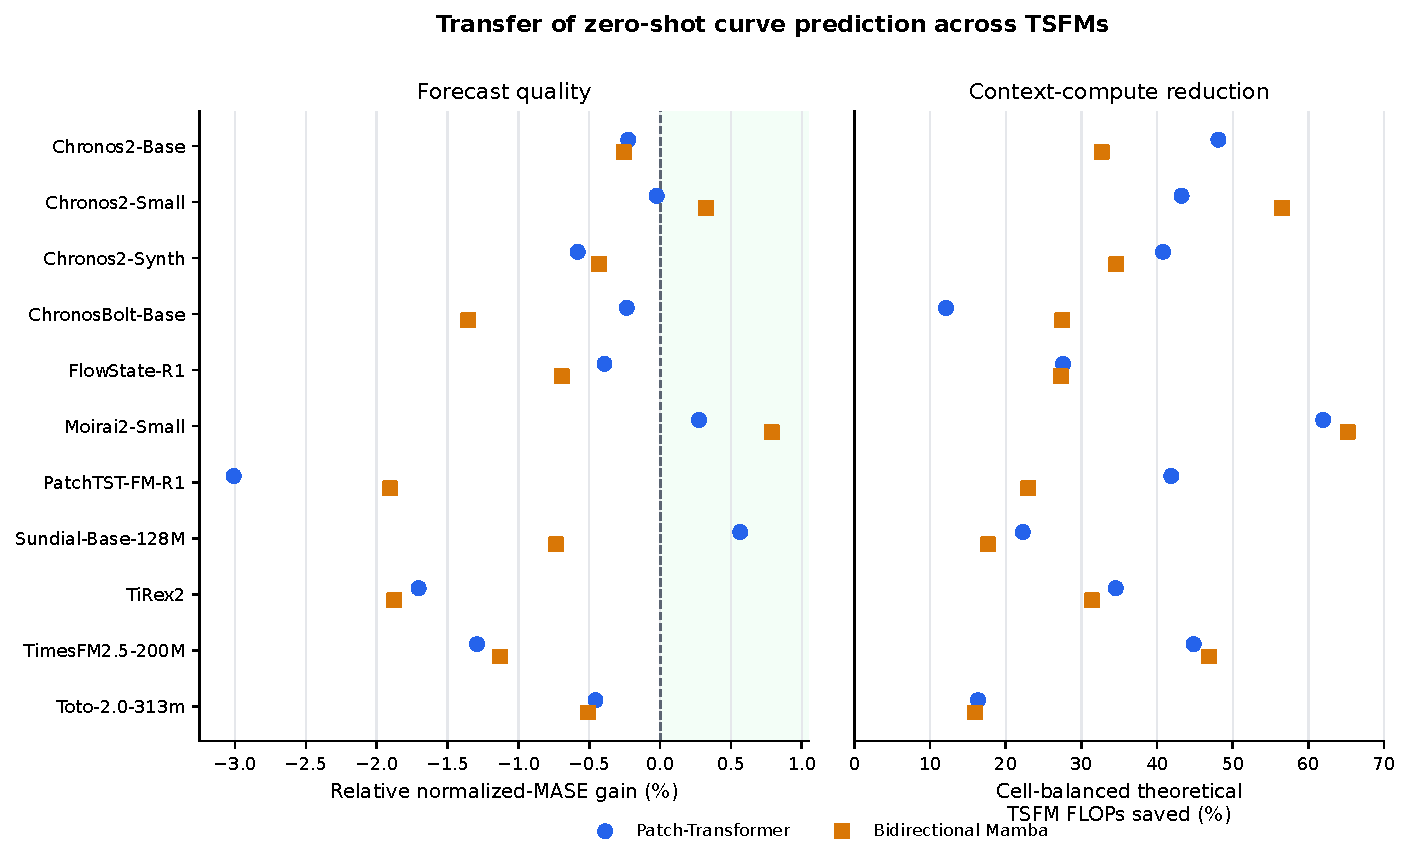
\includegraphics[width=0.96\textwidth]
        {figures/fig3_zero_shot_multimodel.pdf}
    \caption{Transfer of zero-shot curve prediction across 11 TSFMs.  The left panel shows
    relative normalized-MASE gain over native context (positive is better); the
    right shows cell-balanced theoretical TSFM FLOPs saved.  Both the
    Patch-Transformer and Mamba predictors shorten context broadly, while
    accuracy transfer remains forecaster dependent.  TiRex internally pads to a fixed context, so
    its theoretical shortening proxy should not be interpreted as realized
    hardware savings.}
    \label{fig:zero-shot-multimodel}
\end{figure*}

\paragraph{Selection stability.}
The top synthetic checkpoints confirm that model selection is a central part
of the calibration gap.  Across the five best Chronos2-Small Mamba trials,
real normalized MASE ranges from 0.722221 to 0.732506 (mean $0.726533$,
standard deviation $0.003881$), and three beat native.  The best real checkpoint
ranks third by synthetic regret, whereas the synthetic runner-up ranks last on
real data.  Patch-Transformer trials are more concentrated (standard deviation
$0.001612$), but their synthetic winner is again the only checkpoint that does
not improve native.  Synthetic regret is therefore sufficient to define a
reproducible zero-shot rule, but not yet to rank close checkpoints reliably.

\paragraph{Selector overhead.}
The selected Mamba predictors contain 0.53--1.00 million parameters and require
0.033--0.241 GMAC per series in the analytic proxy.  Against one
maximum-window TSFM call at horizon 48, this is $0.092\%$--$2.355\%$ across the
11 models (mean $0.566\%$).  The fraction can be larger for cells whose native
history is much shorter than the model maximum.  Consequently, the FLOPs and
timing values above should be read as savings in the forecasting backbone, not
as a measured end-to-end latency claim; a deployment study must include
predictor batching, data transfer, and aggregation.

\subsection{Implications}
\label{sec:zero-shot-implications}

Synthetic supervision can recover useful real-data accuracy--compute policies:
on Chronos2-Small, all five objectives improve on native context, and on Moirai
the curve predictor combines the largest accuracy gain with the largest FLOPs
reduction.  These gains are obtained without observing a real error curve at
training or selection time.

The cross-model study identifies calibration, rather than action-space
coverage, as the limiting factor.  Synthetic validation regret does not always
rank nearby checkpoints correctly, and the best predictor backbone varies by
forecaster.  In addition, the present policy relies on cell-level aggregation
and requires a model-specific offline labeling sweep.  These are concrete
design constraints rather than evidence against adaptive context selection.

A stronger selector should therefore learn uncertainty over the response
curve, choose sets of regret-bounded actions, and retain native context when
the predicted margin is weak.  The results here establish the central
opportunity: forecast context can be selected from unlabeled inputs to improve
accuracy, reduce compute, or trade between the two.  Achieving that trade-off
consistently across forecasters is the remaining calibration problem.
